% Drawing 154/01-13 -- folder 154, batch 01, archive page 19 (PDF page 20).
% Transcription: figures : en haut, une droite jaune $D$ et, au-dessus, la spécialisation $D'$ en pointillé, qui monte vers le sommet d'un faisceau orange (deux petites flèches verticales, un segment vert sur $D$) ; au bas de la page, la même situation avec les « parallèles » $\widetilde{\widetilde{D}}$, $\widetilde{\widetilde{D}}'$ tracées en pointillé brun, deux flèches désignant les sommets $\sigma$ et $\sigma'$ ; dans la marge, deux petites étoiles de pseudo-droites en $D$ et en $D'$ reliées par une flèche orange, avec les secteurs $\alpha$, $\beta$, $\alpha'$, $\beta'$ et des points $a$, $a'$
% Kind: specialisation of a line towards a vertex; with parallels; marginal stars. Method 2 (redrawn from the facsimile). Status: ok.
% Notes: Three figures, redrawn from the 400 dpi facsimile with every vertex computed once. Top: the yellow line D; a pencil of three orange lines through one vertex (the intersection of the two outer lines, the third drawn through it); the specialisation D' dotted in yellow-green, starting on D and rising through the vertex, down again on the right; the two dark bars across the pencil (dashed blue-green above the vertex, black below it) and the thick blue-green segment just above D, each ending on the two outer lines of the pencil; the two small vertical arrows; further right an orange cross whose two lines meet on D. Foot of the page: D in yellow, two solid brown lines along it (above and below), two dashed brown arcs over the vertex (the outer one from the upper brown line to the upper brown line, the inner one from the lower brown line to the lower brown line, ends computed on those lines); the pencil of three orange lines through one computed vertex, D' dotted in yellow-green from D through the vertex back to D; the three thick black bars are the pieces of the outer arc, of the inner arc and of the upper brown line between the two outer lines of the pencil; arrows to sigma (the bar on the upper brown line) and sigma' (the inner arc); the short blue dotted stroke under the vertex, below the lower brown line, now drawn; an orange cross on the left, a single stroke and a cross on the right, whose lines meet on D. Margin: two small stars of yellow-green pseudolines (each two strands through one vertex, plus a third short stroke at D' under the black arrow a'), joined by the orange arrow from the vertex at D to the vertex at D'; the blue dotted arcs (alpha', beta' at D', alpha, beta at D) drawn as arcs centred on the vertices, from one strand to the other; the yellow dotted ray a' below D on the line from the vertex. The lower marginal point is labelled a' on the facsimile. Doubtful: in the star at D the strands stop short of the vertex on the page and the black point (the tail of the orange arrow) sits a little above where they would meet; the vertex is drawn at their meeting point with the black point on it; a small struck-through scribble left of the star at D is not drawn. Redrawn 2026-11-09 (issue 128): to check again.
% Coordinates: 1 unit = 1 mm = 1/100 of the crop width (bbox in page fractions: [0.121, 0.249, 0.438, 0.531]).
% Redrawn by Claude (claude-opus-5-5), issue #73, 2026-11-07; not checked by a human; not compiled (no TeX in the session).
% Redrawn by Claude (claude-opus-5-5) 2026-11-09 (issue #128, third pass): strands traced one by one on the 400 dpi facsimile (positions read off the colour mask), pairwise crossings checked inside the disk, shared ends computed once, regions bounded by their strands; labels at \small. Not compiled. Status: ok.
% Rights: reproduces part of the work -- behind RENDER_TRANSCRIPTS, never published by itself.
\documentclass[tikz,border=3pt]{standalone}
\usepackage{amsmath,amssymb}
\usetikzlibrary{patterns,arrows.meta}
\tikzset{Or/.style={orange!90!black}, Ye/.style={yellow!80!orange}, Lg/.style={green!60!black!70}, Dg/.style={green!45!black}, Br/.style={brown!80!black}, Rd/.style={red!85!black}, Bl/.style={blue!70!black}, Gy/.style={black!40}, pencil/.style={black!45}, struck/.style={black!35}, mark/.style={circle,draw,inner sep=1.3pt}, pt/.style={circle,fill,inner sep=0.9pt}, opt/.style={circle,draw,fill=white,inner sep=1.1pt}}
\colorlet{Or}{orange!90!black}\colorlet{Ye}{yellow!80!orange}\colorlet{Lg}{green!60!black!70}\colorlet{Dg}{green!45!black}\colorlet{Br}{brown!80!black}\colorlet{Rd}{red!85!black}\colorlet{Bl}{blue!70!black}\colorlet{Gy}{black!40}
\begin{document}
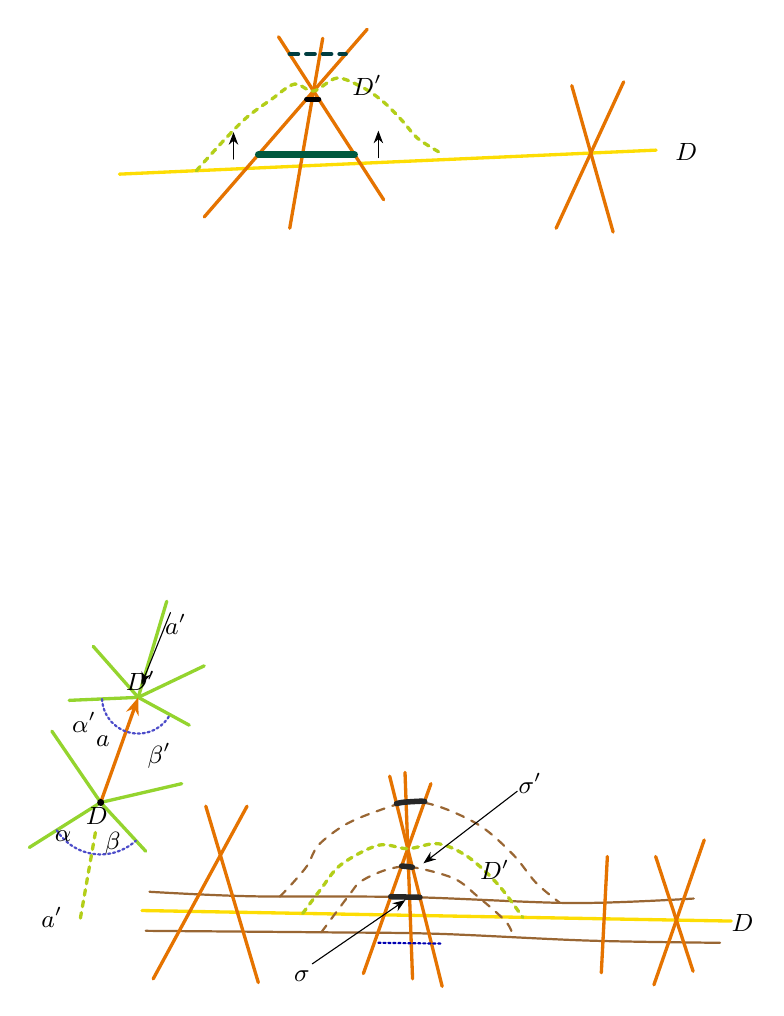
\begin{tikzpicture}[x=1mm,y=1mm,line cap=round,line join=round,font=\scriptsize]
\draw[Br,thick] plot[smooth, tension=0.55] coordinates {(20.5,-112.87) (33.37,-113.44) (53.38,-113.54) (74.36,-114.3) (89.61,-113.73)};
\draw[Br,thick] plot[smooth, tension=0.55] coordinates {(20.02,-117.83) (42.9,-118.02) (57.2,-118.21) (76.26,-119.07) (92.95,-119.35)};
\draw[Ye,very thick] (16.68,-21.73) -- (84.84,-18.68);
\draw[Or,very thick] (27.45,-27.17) -- (48.14,-3.34);
\draw[Or,very thick] (36.89,-4.29) -- (50.24,-24.98);
\draw[Or,very thick] (42.5,-4.48) -- (38.31,-28.6);
\draw[Bl!60!green!60!black,line width=1.6pt,dashed] (38.31,-6.48) -- (45.41,-6.48);
\draw[line width=1.8pt] (40.45,-12.2) -- (42,-12.2);
\draw[Bl!50!green!70!black,line width=2.4pt] (34.32,-19.26) -- (46.55,-19.26);
\draw[Ye!70!green,very thick,dash pattern=on 2pt off 2.2pt] plot[smooth, tension=0.55] coordinates {(26.44,-21.3) (30.03,-17.35) (32.89,-14.49) (36.03,-12.2) (38.89,-10.3) (41.34,-11.18) (44.33,-9.53) (47.66,-10.77) (50.24,-12.58) (52.62,-14.97) (54.53,-17.16) (57.2,-18.88)};
\draw[-{Stealth[length=1.6mm]}] (31.17,-19.83) -- (31.17,-16.4);
\draw[-{Stealth[length=1.6mm]}] (49.57,-19.64) -- (49.57,-16.21);
\node[inner sep=1pt] at (48.14,-10.49) {\small $D'$};
\draw[Or,very thick] (74.13,-10.49) -- (79.38,-29.08);
\draw[Or,very thick] (80.72,-10.01) -- (72.14,-28.6);
\node[inner sep=1pt] at (88.66,-18.88) {\small $D$};
\draw[Ye,very thick] (19.54,-115.25) -- (94.38,-116.59);
\draw[Or,very thick] (51,-98.19) -- (57.67,-124.88);
\draw[Or,very thick] (56.24,-99.14) -- (47.66,-123.26);
\draw[Or,very thick] (52.95,-97.71) -- (53.91,-123.93);
\draw[Br,thick,dashed] plot[smooth, tension=0.55] coordinates {(37.06,-113.49) (38.89,-111.53) (40.61,-109.44) (41.94,-106.96) (45.28,-104.39) (49.29,-102.67) (53.67,-101.43) (57.67,-102.19) (62.63,-104.58) (66.73,-108.2) (69.59,-111.73) (72.62,-114.28)};
\draw[Br,thick,dashed] plot[smooth, tension=0.55] coordinates {(42.33,-118.01) (45.95,-113.16) (47.38,-111.53) (50.52,-110.1) (53.67,-109.72) (59.1,-111.15) (62.15,-113.44) (65.78,-116.68) (66.72,-118.64)};
\draw[black!85,line width=2pt] (51.87,-101.67) -- (51.91,-101.66) -- (51.96,-101.64) -- (52.02,-101.63) -- (52.08,-101.62) -- (52.14,-101.6) -- (52.2,-101.59) -- (52.27,-101.58) -- (52.34,-101.56) -- (52.41,-101.55) -- (52.48,-101.54) -- (52.55,-101.53) -- (52.63,-101.52) -- (52.7,-101.51) -- (52.79,-101.5) -- (52.87,-101.49) -- (52.96,-101.48) -- (53.05,-101.47) -- (53.14,-101.47) -- (53.24,-101.46) -- (53.34,-101.45) -- (53.45,-101.44) -- (53.56,-101.44) -- (53.67,-101.43) -- (53.78,-101.42) -- (53.89,-101.42) -- (53.99,-101.41) -- (54.09,-101.41) -- (54.19,-101.4) -- (54.28,-101.4) -- (54.36,-101.39) -- (54.44,-101.39) -- (54.52,-101.38) -- (54.6,-101.38) -- (54.67,-101.38) -- (54.74,-101.38) -- (54.8,-101.37) -- (54.86,-101.37) -- (54.92,-101.37) -- (54.98,-101.37) -- (55.03,-101.37) -- (55.09,-101.37) -- (55.14,-101.37) -- (55.19,-101.38) -- (55.23,-101.38) -- (55.28,-101.38) -- (55.32,-101.39) -- (55.37,-101.39) -- (55.41,-101.4) -- (55.44,-101.4);
\draw[black!85,line width=2pt] (52.52,-109.6) -- (52.54,-109.6) -- (52.6,-109.6) -- (52.67,-109.61) -- (52.74,-109.62) -- (52.81,-109.62) -- (52.89,-109.63) -- (52.97,-109.64) -- (53.06,-109.65) -- (53.15,-109.66) -- (53.24,-109.67) -- (53.34,-109.68) -- (53.45,-109.7) -- (53.55,-109.71) -- (53.67,-109.72) -- (53.79,-109.74) -- (53.89,-109.75);
\draw[black!85,line width=2pt] (51.14,-113.49) -- (51.28,-113.5) -- (51.78,-113.51) -- (52.29,-113.51) -- (52.83,-113.53) -- (53.38,-113.54) -- (53.94,-113.55) -- (54.47,-113.56) -- (54.85,-113.57);
\draw[Ye!70!green,very thick,dash pattern=on 2pt off 2.2pt] plot[smooth, tension=0.55] coordinates {(39.96,-115.62) (42.23,-112.58) (44.8,-109.44) (49.57,-106.96) (53.3,-107.4) (57.2,-106.77) (61.01,-108.48) (64.82,-112.01) (67.9,-116.12)};
\draw[Bl,densely dotted,thick] (49.57,-119.35) -- (57.67,-119.45);
\draw[Or,very thick] (27.65,-102) -- (34.32,-124.4);
\draw[Or,very thick] (32.89,-102) -- (20.97,-123.93);
\draw[Or,very thick] (78.65,-108.39) -- (77.88,-123.16);
\draw[Or,very thick] (84.78,-108.39) -- (89.54,-122.97);
\draw[Or,very thick] (90.95,-106.29) -- (84.56,-124.69);
\node[inner sep=1pt] at (95.81,-116.78) {\small $D$};
\draw[-{Stealth[length=1.6mm]}] (41.18,-122.02) -- (53,-113.92);
\node[inner sep=1pt] at (39.85,-123.55) {\small $\sigma$};
\draw[-{Stealth[length=1.6mm]}] (67.21,-100.1) -- (55.29,-109.25);
\node[inner sep=1pt] at (68.83,-99.14) {\small $\sigma'$};
\node[inner sep=1pt] at (64.35,-110.1) {\small $D'$};
\draw[Lg!60!yellow,very thick] (10.3,-88.56) -- (19.07,-88.18) -- (27.45,-84.18);
\draw[Lg!60!yellow,very thick] (13.35,-81.7) -- (19.07,-88.18) -- (25.55,-91.71);
\draw[Lg!60!yellow,very thick] (8.1,-92.47) -- (14.3,-101.53) -- (20.02,-107.72);
\draw[Lg!60!yellow,very thick] (5.24,-107.24) -- (14.3,-101.53) -- (24.59,-99.14);
\draw[Lg!60!yellow,very thick] (22.69,-75.98) -- (19.07,-88.18);
\draw[-{Stealth[length=1.6mm]}] (23.16,-77.41) -- (19.47,-86.58);
\draw[Or,very thick,-{Stealth[length=2.2mm]}] (14.3,-101.53) -- (19.07,-88.18);
\node[pt] at (14.3,-101.53) {};
\draw[Ye!70!green,very thick,dash pattern=on 2pt off 2.2pt] (13.63,-105.34) -- (11.63,-116.78);
\draw[Bl!70,densely dotted,thick] (14.47,-88.38) arc[start angle=-177.51, end angle=-28.55, x radius=4.6, y radius=4.6];
\draw[Bl!70,densely dotted,thick] (8.72,-105.05) arc[start angle=-147.72, end angle=-47.29, x radius=6.6, y radius=6.6];
\node[inner sep=1pt] at (19.35,-86.08) {\small $D'$};
\node[inner sep=1pt] at (12.2,-91.33) {\small $\alpha'$};
\node[inner sep=1pt] at (14.59,-93.71) {\small $a$};
\node[inner sep=1pt] at (21.73,-95.61) {\small $\beta'$};
\node[inner sep=1pt] at (13.82,-103.24) {\small $D$};
\node[inner sep=1pt] at (9.53,-105.82) {\small $\alpha$};
\node[inner sep=1pt] at (15.82,-106.77) {\small $\beta$};
\node[inner sep=1pt] at (8.1,-116.11) {\small $a'$};
\node[inner sep=1pt] at (23.83,-78.93) {\small $a'$};
\end{tikzpicture}
\end{document}
